% @Author: Xiaocheng Tang
% @Date:   2017-05-11 22:01:21
% @Last Modified by:   Xiaocheng Tang
% @Last Modified time: 2017-05-11 22:02:26
% !TEX root = ./abstract.tex

In this work we utilize generative models to create new training labels and de-noise the data (\cite{genmodels}).
The model applies generative processes to labeling functions and learns their structural correlations and conflicts.
We incorporate numerous labeling functions as a supply of domain knowledge for weak supervision. Table (\ref{tab:numrules})
lists some of the categories and the number of rules associated with them. Labeling functions assign 1 if the product belongs
to the category, -1 if it does not and 0 if it is uncertain\cite{genmodels}.

The generative model optimizes noise aware loss function and estimates probabilities $p(Label, \lambda)$,
where $Label$ is the category we want to predict, $\lambda = f(x)$ is a list of values assigned by labeling
functions $f$ to product $x$.

Since current implementation of generative model is binary, we apply it to each
category separately and combine the results in a final output. Picture (\ref{fig:genmodel_pred_probs}) shows
the distribution of marginal probabilities for several classes. We assume that the product belongs to certain category if
prediction probability is greater or equal to 0.5.

We use unlabeled product items to train generative model and apply learned model to manually labeled test data and measure
prediction accuracy (\ref{tab:evaluation}).
The train and test sets contain respectively 100k and 20k product items.
'Boots \textgreater Women' category contains 88 rules with very small overlap, whereas 'Boots \textgreater Men' category
has less rules but more overlaps and conflicts. Despite of the noise and rule conflicts the model is able to learn from rules with high accuracy (\ref{tab:evaluation}).

In addition, we demonstrate the fraction of coverage, overlaps and conflicts in table (\ref{tab:overlapconflict}). The results show that despite
of the small rules coverage in the presence of conflicts and overlaps the system is able to generalise and de-noise the data.

Ultimately, we combine generated and manually labeled training sets to train a discriminative model to predict accurate product categories.

\begin{table*}
  \caption{Examples of the category labels and the total numbers of rules in each category}
  \label{tab:numrules}
  \begin{tabular}{ll}
    \toprule
    Category & \#Rules\\
    \midrule
    Boots \textgreater Women &	88	\\
    Boots \textgreater Men	& 36 \\
 	Travel \textgreater Hotel & 30 \\
 	Home \textgreater LampShades & 19 \\
 	Home \textgreater Other & 11 \\
 	Grocery \textgreater Nutrition Drinks & 11 \\
    \bottomrule
  \end{tabular}
\end{table*}

\begin{table*}
  \caption{Evaluation results for several categories on sub-sampled data}
  \label{tab:evaluation}
  \begin{tabular}{lllllll}
    \toprule
    Category & Presicion & Recall & F1 & Accuraccy & Neg Class Accuracy & Pos Class Accuracy\\
    \midrule 
    Boots \textgreater Women	& 93\% & 96\% & 94\% & 99\% & 96\% & 93\% \\
    Boots \textgreater Men &	60\%	& 75\% & 66\% & 99\% & 75\% & 60\% \\
    \bottomrule
  \end{tabular}
\end{table*}

\begin{table*}
  \caption{The coverage, overlaps and conflicts for a fraction of rules from 'Boots \textgreater Men' category}
  \label{tab:overlapconflict}
  \begin{tabular}{llll}
    \toprule
    Rule Label & Coverage & Overlaps & Conflicts \\
    \midrule
    Regexp_1	& 0.003050 & 0.003025 & 0.000025 \\
    Regexp_2	& 0.148550 & 0.007500 & 0.000125 \\
    Regexp_3	& 0.067900 & 0.002650 & 0.000100 \\
    Regexp_4	& 0.783975 & 0.007050 & 0.000100 \\
    ... \\
    Regexp_{35}	& 0.008150 & 0.002400 & 0.000100 \\
    Regexp_{36}	& 0.020120 & 0.016793 & 0.000000 \\
    \bottomrule
  \end{tabular}
\end{table*}

\begin{figure}[th]
   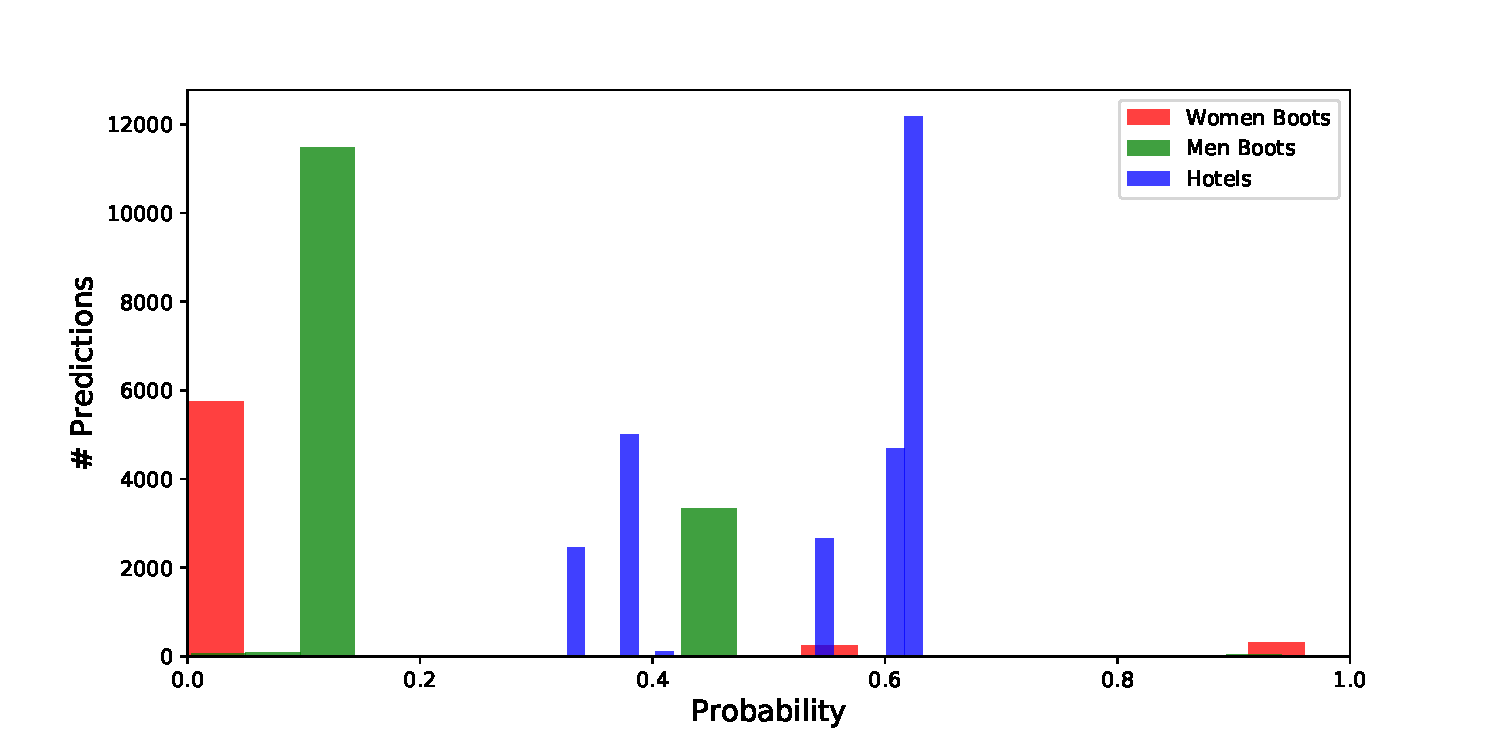
\includegraphics[width=0.5\textwidth]{resources/genmodel_pred_probs}
   \caption{The distribution of marginal probabilities}
   \label{fig:genmodel_pred_probs}
   \centering
\end{figure}


/*
weak supervision, in which training labels are noisy and may be from
multiple, potentially overlapping sources
To address this, we model the labeling functions as a generative
process, which lets us automatically de-noise the resulting training set by learning the accuracies of
the labeling functions along with their correlation structure. In turn, we use this model of the training
set to optimize a stochastic version of the loss function of the discriminative model that we desire to train. 
*/